\chapter{État de l’art}

\section{Introduction}

Comme cité précédemment, les écrans géants sont une technologie qui tend à se répandre et à être de plus en plus présent dans notre environnement. Cependant l'utilisation et l'appréhension de cet outil est différent de ce que l'on peut rencontrer actuellement sur des écrans dits classiques. Notre étude des écrans géants se porte sur l'amélioration du confort visuel pour un utilisateur en fonction de sa distance avec l'écran. En effet, en fonction de la distance qui sépare l'utilisateur de l'écran, l'interaction et le ressenti visuel sont différents. Sur une interaction dite proche un effet de perspective apparaît et devient gênant pour interagir avec les widgets visibles sur l'écran. Sur une interaction éloignée la densité d'information visuelle est un inconvénient pour une interaction précise.

\section{Interaction proche sur grand écran}

\subsection{Effet de perspective}

La perspective est l'un des indices visuels qui nous permet de représenter le monde qui nous entoure. La perspective est un ensemble de règles énoncées par \textit{Filippo Brunelleschi} qui permet de représenter une image sur une surface plane tout en ayant l'impression de réalité grâce à des lignes de fuite. Les lignes sont des ensembles de points qui représentent la direction du plan visualisé. Celles-ci sont présentes lorsque l'on regarde un écran géant de près et donne un rendu étiré de l'image qui est affichée dans notre cas, sur l'écran géant. Voici un aperçu de ce qu'est l'effet de perspective rencontré face à une surface plane, voire figure \ref{fig:perspectiveScreen}, ce qui est également ce qu'on obtient face aux écrans géants.

\begin{figure}[!ht]
	\center	
	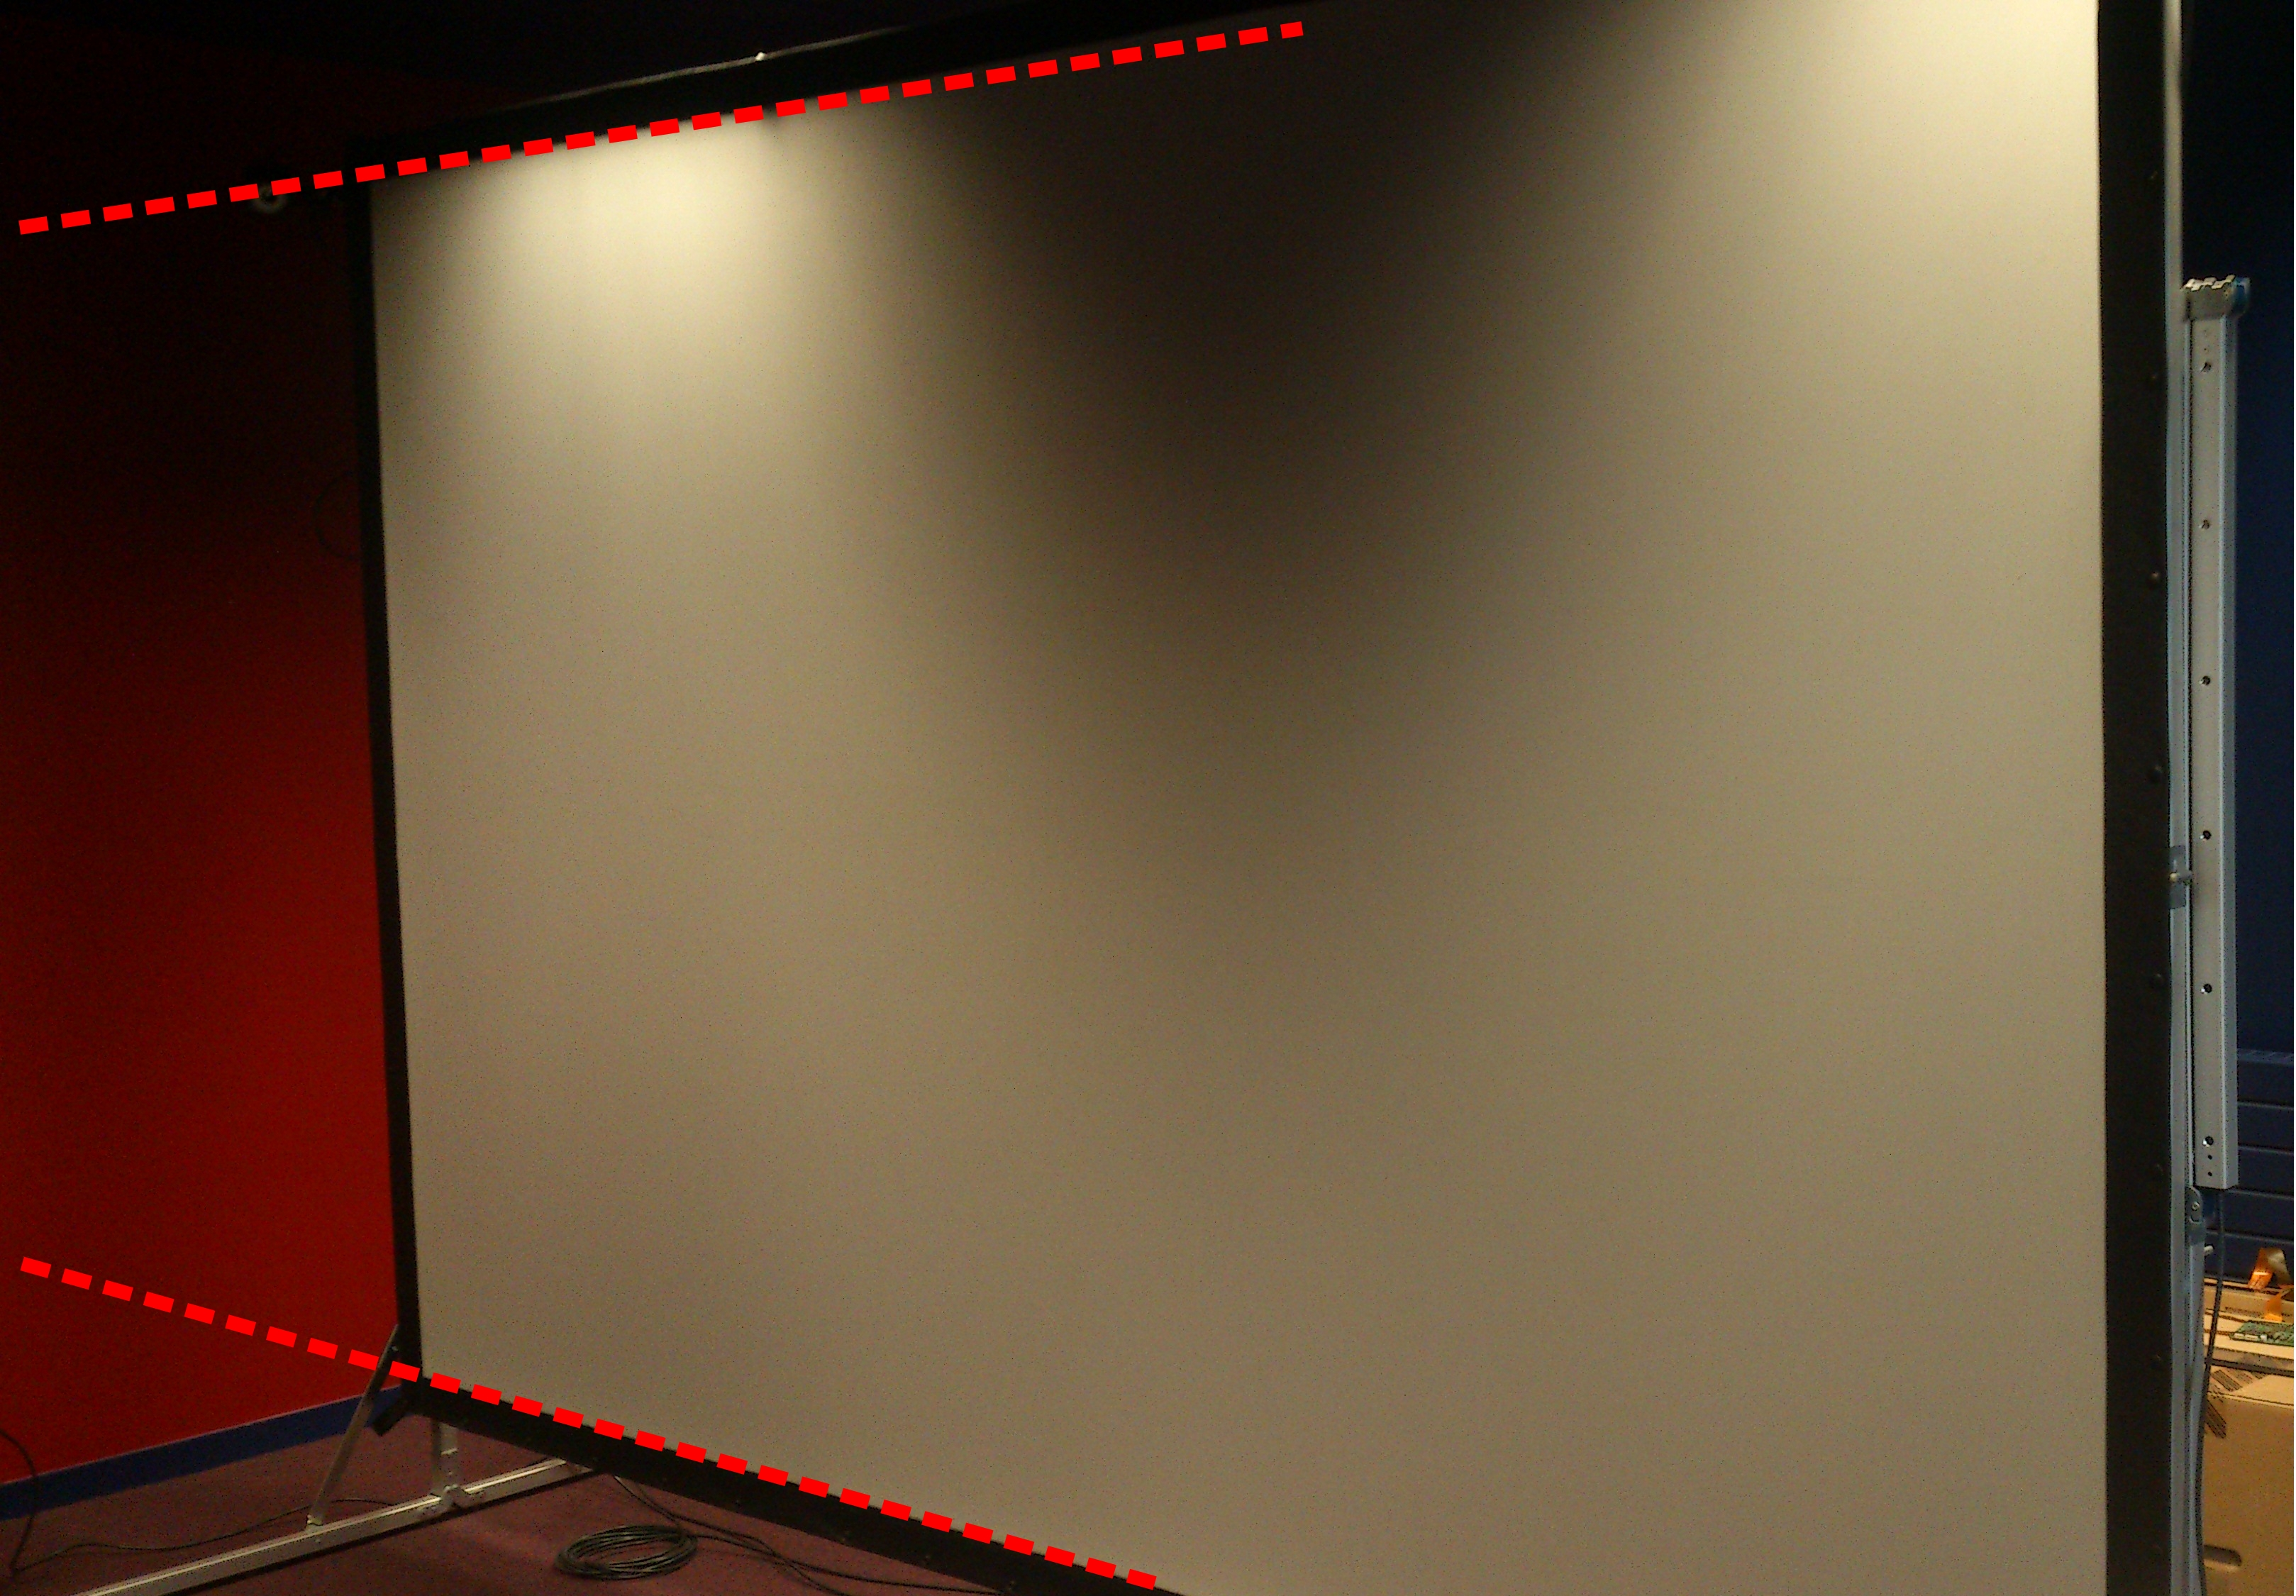
\includegraphics[scale=0.1]{image/perspectiveScreen.jpg}
	\caption{Effet de perspective visible face à un écran géant}
	\label{fig:perspectiveScreen}
\end{figure}

L'effet de perspective est un sujet qui a été traité dans de nombreux cas comme par exemple avec Econics \cite{Nacenta:2007:EPI:1294211.1294260} qui traitait le problème de l'effet de perspective par une déformation statique des fenêtres de l'environnement. 

\subsection{Correction de la perspective}


Econics voire figure \ref{fig:econics}, est un prototype permettant de définir plusieurs écrans situé a des emplacements et orientation aléatoire tout en proposant pour l'utilisateur un retour visuel de son application orthogonal par rapport à son point de vue et non par rapport à l'écran.

\begin{figure}[!ht]
	\center	
	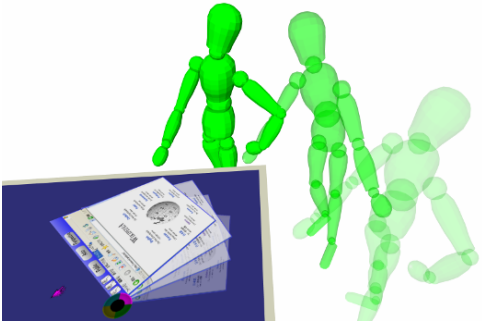
\includegraphics[scale=0.5]{image/econics.png}
	\caption{Aperçu de la correction de perspective d'Econics}
	\label{fig:econics}
\end{figure}

Comme Econics l'a fait pour corriger l'effet de perspective, il est possible de modifier la géométrie des fenêtres affichées de façon indépendante les unes des autres. Econis fait une déformation dynamique des fenêtres en fonction du point de vue utilisateur. La déformation de la fenêtre sur fait autour d'un point d'ancrage 3D que l'utilisateur définit. Econics introduit donc une base à la correction de la perspective cependant il a été conçu pour répondre à la problématique de la correction de perspective sur plusieurs écrans de taille normale dispersés dans une pièce et non un unique écran géant. 
%% il y a une déformation dynamique fonction du pt de vue utilisateur indé pour chaque fenetre. Chaque fenetre tourne autour d'un point d'acnreage 3D définit pour l'utilisateur OK

La correction de perspective a également été mise en place pour le prototype Screenfinity \cite{Schmidt:2013:SEP:2470654.2466227} réalisé par Schmidt et al. . L'objectif de Screenfinity est d'afficher du texte déformé sur un écran géant pour que les passants puissent lire le texte tout en marchant et sans l'effet de perspective, voire figure \ref{fig:screenfinity}. Screenfinity utilise donc la déformation dynamique d'image en tenant compte de la position des passants et de leurs orientation de tête. Pour calculer la déformation à appliquer, la position et l'orientation des passant sont pris en compte. Cette déformation de l'image prend en considération les caractéristiques de la vision humaine.
%% Cette déformation prend en compte les caractéristiques de la vision humaine
%Pour calculer la déformation à appliquer en fonction de la position et l'orientation des passant, il faut tenir compte de l'acuité visuelle. OK

\begin{figure}[!ht]
	\center	
	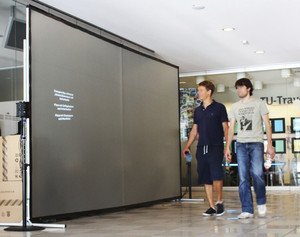
\includegraphics[scale=1]{image/screenfinity.jpg}
	\caption{Aperçu de Screenfinity et de sa correction de perspective en fonction du regard des passants}
	\label{fig:screenfinity}
\end{figure}


\subsection{Méthode de déformation d'affichage}

L'une des méthode générique de déformation d'image est l'anamorphose découverte fin du quinzième siècle dans le milieu de l'art tant pour ajouter du challenge aux artistes que pour confirmer leurs maîtrises de la perspective qui fût découverte en même temps.
Une anamorphose est une déformation réversible d'une image à l'aide d'un système optique, tel un miroir courbe, ou un procédé mathématique.

L'une des plus célèbres anamorphoses est celle réalisée par Hans Holbein sur la toile \textit{Les ambassadeurs}, voir \ref{fig:ambassador}.

\begin{figure}[!ht]
    \centering
    \subfigure[]{\label{sub1} 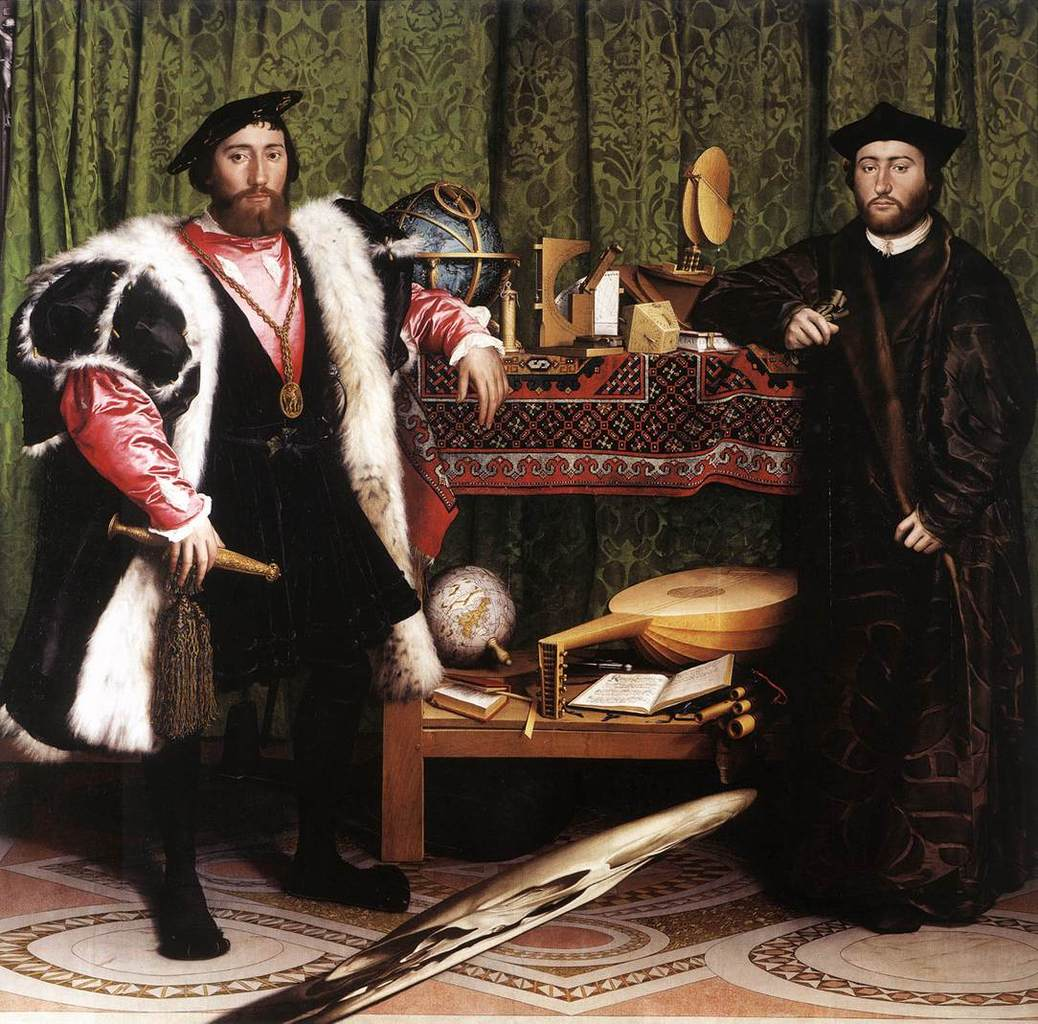
\includegraphics[scale=0.7]{image/ambassador.jpg}}
    \subfigure[]{\label{sub2} 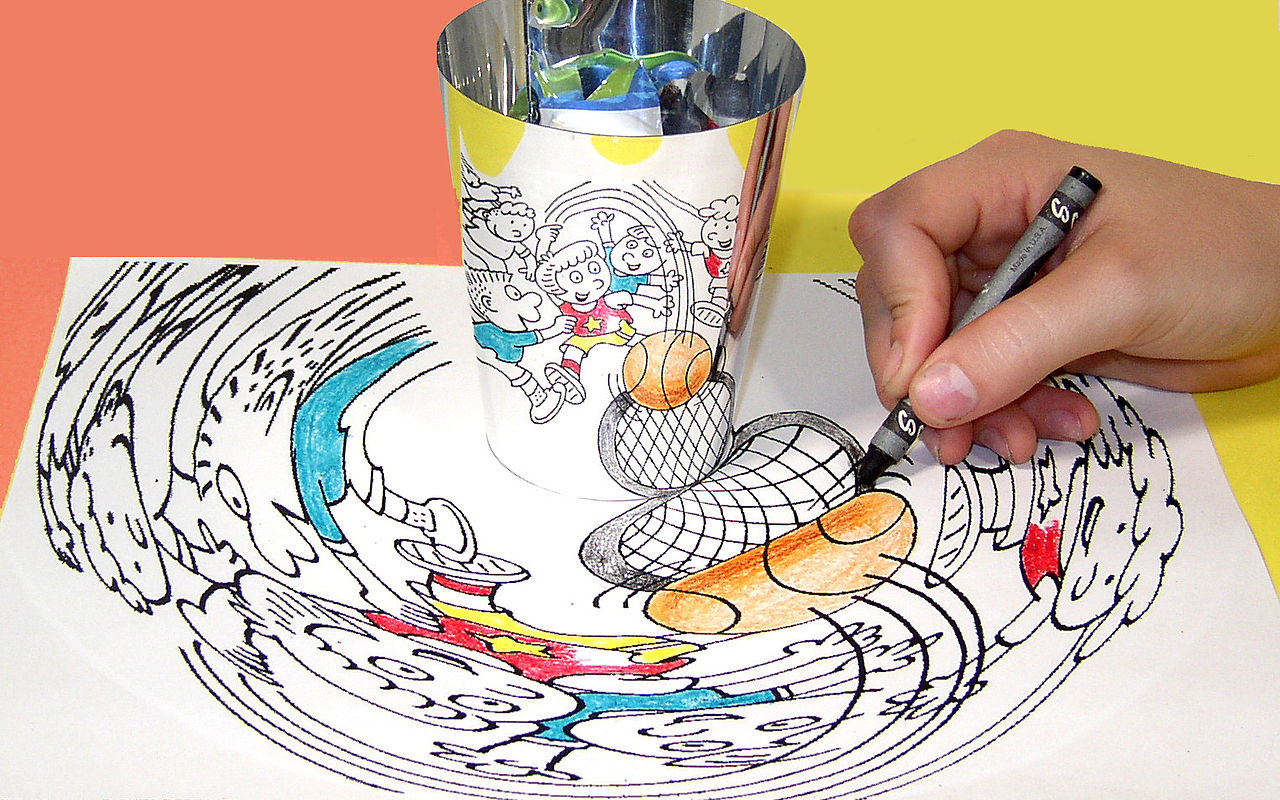
\includegraphics[scale=0.2]{image/anamorphose}}
    \caption{Les ambassadeurs de Hans Holbein le Jeune, 1533 \subref{sub1},  anamorphose avec miroir cylindrique \subref{sub2}.}
	\label{fig:ambassador}
\end{figure}

Sur cette toile, on peut voir apparaître une forme étrange sur le bas de ce tableau, il s'agit d'une anamorphose d'un crâne humain. Si on regarde le tableau depuis le côté inférieur gauche du tableau, le crane est visible correctement. L'anamorphose est présente sur plusieurs supports, comme par exemple dessiné par des artistes dans certaines rues \cite{pavementArt}.

%% enlever premiere et derniere OK
L’aspect dynamique de l’anamorphose consiste à ne pas appliquer une déformation statique de l’image, pour laquelle il faut se placer à un point de vue particulier pour obtenir visuellement l'image non déformée, mais déformer l’image en temps réel en tenant compte de paramètres, tels que la position de l’utilisateur face a l’image, pour que celle-ci soit déformée mais parfaitement visible pour l'utilisateur. 

L'anamorphose dynamique introduite par Solina et al. est de la distorsion d'image pour afficher des visages tout en ayant l'impression que le regard des portraits est dirigé vers l'utilisateur. Nous reprendrons donc l'idée de la déformation dynamique sans conserver l'objectif de Solina et al. qui était de garder la direction du regard du portrait vers l'utilisateur.










\section{Interaction distante sur grand écran}
%%changer le titre pour perception humaine OK
\subsection{Perception humaine}

L'acuité visuelle est la mesure de la résolution spatiale du processus visuel, autrement dit de l'œil humain. La vision binoculaire est un mode de vision dans lequel les deux yeux sont utilisés simultanément \ref{fig:acuite}. 

\begin{figure}[!ht]
	\center	
	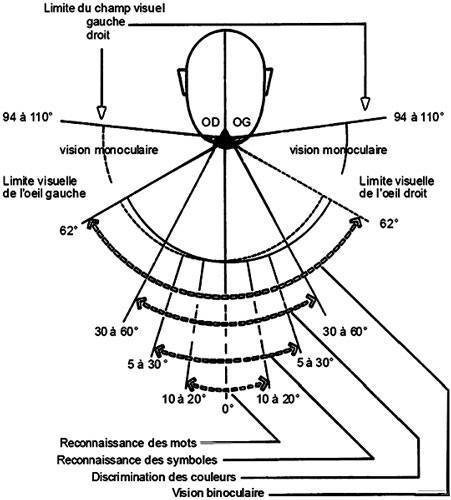
\includegraphics[scale=0.4]{image/acuite.jpg}
	\caption{Représentation des différents champs de vision de l'être humain.}
	\label{fig:acuite}
\end{figure}
%% elevé du détail sur chaque oeil, juste préciser le 120 binoculaire + capacité vison de détail OK
Les humains ont un champ de vision horizontal maximal de $\simeq$120\degres  environ avec les deux yeux. La vision humaine est également limité en terme de perception des détails. En moyenne un œil humain n'arrive pas à percevoir une différence au delà de 76 dpi à une distance de un mètre, et au delà de 38 dpi pour une distance de deux mètres. Il faut donc tenir compte de la vision humaine lorsque l'on fait de l'affichage.

%% changer : la vision humaine doit être prise en compte lorsque l'on fait de l'affichage. OK
%L'acuité visuelle est également importante dans le cas ou la densité d'affichage est élevé et que l'on souhaite lire à distance des informations. 


Comme dit précédemment les écrans sont de plus en plus grands et leurs résolutions sont également de plus en plus élevées. Trois problèmes liés à l'augmentation du nombre de pixel présent par unité d'espace, autrement appelé pixel per inch (ppi) sont présentés selon Agarwal et al. \cite{Agarwal:2013:WSA:2578048.2578052}. Sur les trois problèmes identifiés deux nous concernent directement pour l'utilisation distante des grands écrans.

Le premier problème étant que la plupart des applications, les systèmes d'exploitation et plus généralement les interfaces graphiques ne sont pas adaptés pour des résolutions élevées. Ce fut le cas des écrans "Retina" (220 ppi) d'Apple qui ont dû forcer certaines applications à se mettre à jour car inadapté pour une telle résolution, habituellement comprise entre 72 et 110 dpi. Ensuite vient le problème lié à la vision des utilisateurs. En effet les utilisateurs ayant des troubles de la vision, tels que les daltoniens ou encore les personnes âgées, souffrent des mêmes problèmes face à des écrans avec de grandes résolutions d'affichages. Ces problèmes sont des incapacités à lire correctement du texte, une imprécision sur l'ensemble des images affichées à l'écran, ou encore une incapacité à interagir avec des widgets trop petits.

En effet, comme expliqué dans cet article \cite{Nancel:2013:HPL:2470654.2470773} qui traite d'une technique d'interaction pour grands écrans, lorsqu'il y a interaction directe avec l'écran la zone sous le doigt correspond a une douzaine de pixel. On imagine bien que le problème du pointage à distance qui en plus d'être imprécis, apporte encore plus de difficultés pour interagir avec une zone comportant énormément de pixels.
          
\subsection{Zoom global}


Pour palier à ces problèmes d'affichage trop petit une solution fut d'utiliser les loupes \cite{Kline:1995:IGA:223904.223919}, autrement appelées magnifying glass.

\begin{figure}
    \centering
    \subfigure[]{\label{sub1} 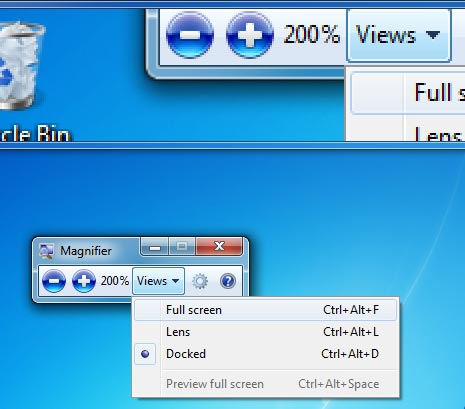
\includegraphics[scale=0.4]{image/loupeWindows.jpg}}
    \subfigure[]{\label{sub2} 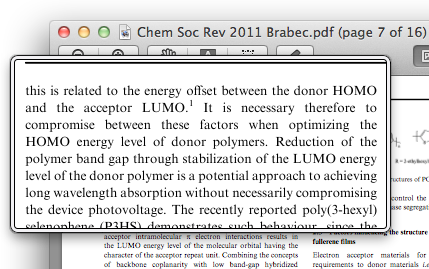
\includegraphics[scale=0.4]{image/loupeMac.png}}
    \caption{Aperçu des loupes implémentés dans \subref{sub1}Windows et \subref{sub2}Mac OS X.}
	\label{fig:loupeDemo}
\end{figure}

Parmi les loupes existantes et implémentées dans les systèmes d'exploitation modernes, la plupart occupent l'ensemble de l'écran ou cachent certaines parties autour de la loupe, voir figure \ref{fig:loupeDemo}. Cela à pour effet de perdre une partie des informations se trouvant sous les bords de la loupe. Pour les loupes qui occupent une plus grande partie de l'écran, cela a pour effet de perdre encore plus d'informations car si l'utilisateur n'a pas connaissance de son environnement graphique, il doit parcourir l'ensemble de l'écran pour pouvoir s'y repérer et interagir. 


\subsection{Zoom local}

Pour garder une vue globale de l'environnement graphique de nombreuses loupes ont étés expérimentés \cite{Carpendale:2004:AHM:1029632.1029645}, voire un aperçu des loupes figure \ref{fig:loupeMultiple}. Ces loupes permettent de faire un zoom sur l'image sans cacher l'information autour ou en dessous du zoom. Ce sont des zooms de type local.


\begin{figure}[!ht]
	\center	
	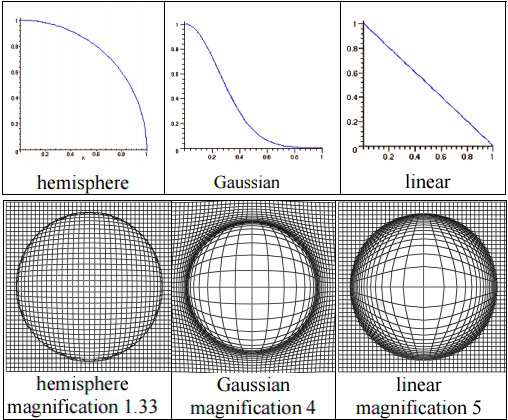
\includegraphics[scale=0.7]{image/LoupeMultiple.png}
	\caption{Aperçu de différents types de loupe}
	\label{fig:loupeMultiple}
\end{figure}

% demo fisheye
L'une des loupes qui ré-apparaît souvent dans la littérature est la loupe fisheye, voire figure \ref{fig:fisheyeMap}

\begin{figure}[!ht]
	\center	
	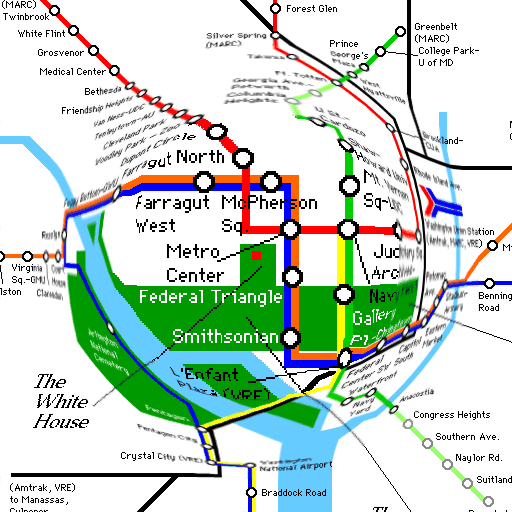
\includegraphics[scale=0.4]{image/fisheyeMap.png}
	\caption{Carte avec rendu fisheye}
	\label{fig:fisheyeMap}
\end{figure}

Dans le domaine de l'interaction homme machine la question du zoom fisheye a souvent été étudié \cite{Shneiderman:1986:DUI:6682, Ware:1995:DIM:223355.223749, Cockburn:2009:ROZ:1456650.1456652} et mis en avant pour montrer l'avantage de cette technique en ce qui concerne la mise en focus de certains éléments. L'une de ses utilisations la plus connue est sur le dock de max OS X, qui est un menu zoomable. L'effet fisheye est une distorsion de l'image qui apporte un gain de performance \cite{Bederson:2000:FM:354401.354782, Furnas:1999:FVN:300679.300769, Gutwin:2002:IFT:503376.503424, Gutwin:2003:FGL:642611.642648} lorsque l'utilisateur souhaite parcourir des données et se concentrer sur une de ces données. Cependant lors d'une sélection, l'effet de distorsion affecte positivement le nombre d'erreurs \cite{Gutwin:2002:IFT:503376.503424}. L'effet fisheye apporte donc une loupe dite contextuelle.


\begin{figure}[!ht]
	\center	
	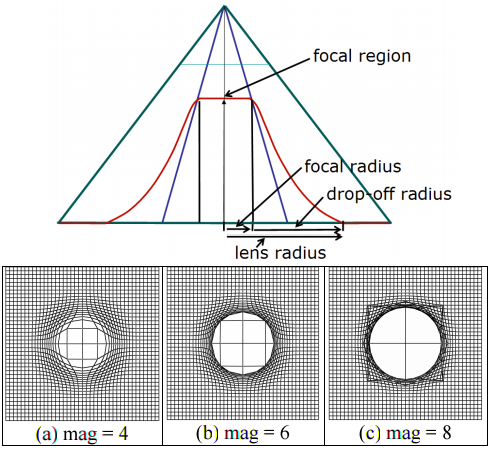
\includegraphics[scale=0.7]{image/LoupeLecture.png}
	\caption{Un aperçu d'une loupe dite de lecture}
	\label{fig:loupeLecture}
\end{figure}

Un des autres types de loupes souvent mis en avant est la loupe dite de lecture. Cette loupe comme visible dans la figure \ref{fig:loupeDemo}, est souvent bornée et cache une partie des informations comme expliqué ci-dessus. On peut voire dans la figure \ref{fig:loupeLecture} un aperçu de ce à quoi peut correspondre une loupe de lecture. On y voit une distorsion d'image sur les bords de la loupe et un ratio fixe de déformation appliqué autour du centre de la loupe (focal region), contrairement aux autres loupes local. Le centre de la loupe fixé et non déformé permet de s'approcher de ce qui est fait aujourd'hui avec des loupes de lecture qui cachent une partie de l'image.

\section{Discussion}

% petit parapgraphe qui reprend les problematiques
% systeme de tracking + deformation
% systeme fisheye a mettre en place
% adapoter l'interaction a la deformation










%
%
%\section{Effet de perspective} 
%
%La perspective est l'un des indices visuels qui nous permet de représenter le monde qui nous entoure. La perspective est un ensemble de règles énoncées par \textit{Filippo Brunelleschi} qui permet de représenter une image sur une surface plane tout en ayant l'impression de réalité grâce à des lignes de fuite. Les lignes sont des ensembles de points qui représentent la direction du plan visualisé. Celles-ci sont présentes lorsque l'on regarde un écran géant de près et donne un rendu étiré de l'image qui est affichée dans notre cas, sur l'écran géant. Voici un aperçu de ce qu'est l'effet de perspective rencontré face à une surface plane, voir \ref{fig:perspectiveScreen}, ce qui est également ce qu'on obtient face aux écrans géants.
%
%\begin{figure}[!ht]
%	\center	
%	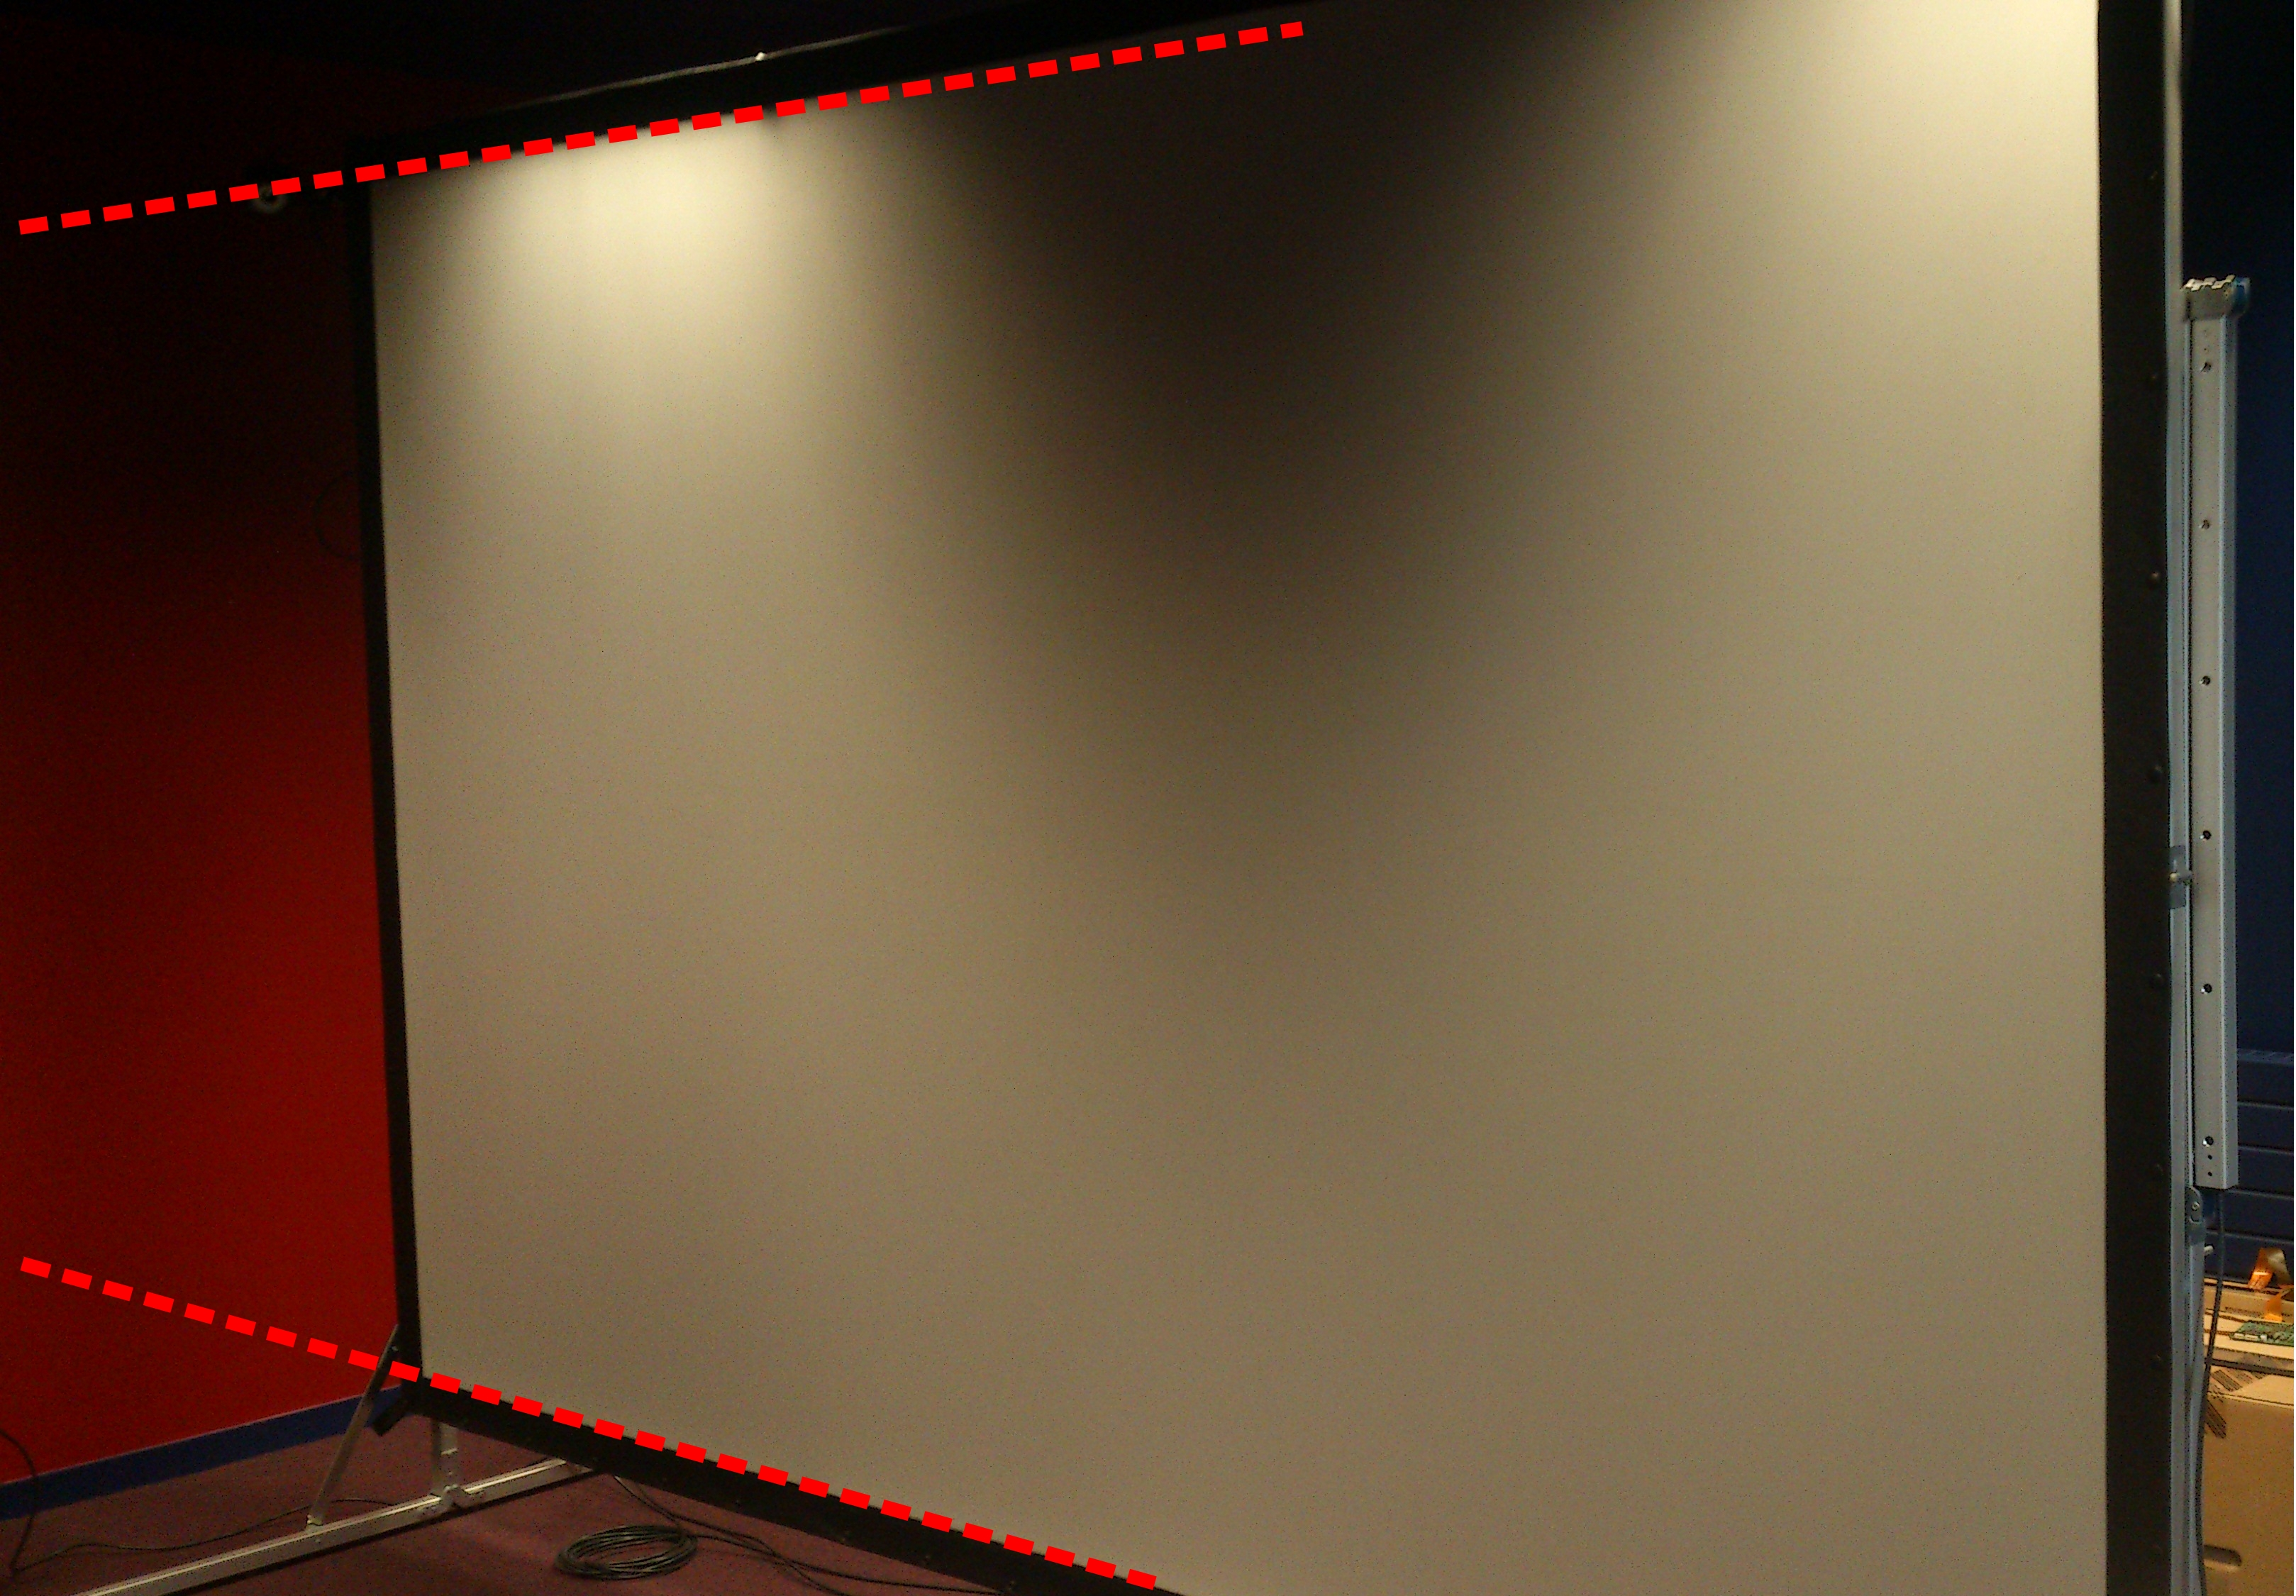
\includegraphics[scale=0.1]{image/perspectiveScreen.jpg}
%	\caption{Effet de perspective visible face à un écran géant}
%	\label{fig:perspectiveScreen}
%\end{figure}
%
%L'effet de perspective est un sujet qui a été traité dans de nombreux cas comme par exemple avec Econics \cite{Nacenta:2007:EPI:1294211.1294260}. Econics est un prototype permettant de définir plusieurs écrans situé a des emplacements et orientation aléatoire tout en proposant pour l'utilisateur un retour visuel de son application orthogonal par rapport à son point de vue et non par rapport à l'écran. Pour réaliser cet effet, ils ont modifié l'apparence visuelle des applications pour corriger l'effet de perspective.
%
%Comme Econics l'a fait pour corriger l'effet de perspective, il est possible de modifier la géométrie des fenêtres affichées de façon indépendante les unes des autres. Une autre solution pour corriger l'effet de perspective serait de déformer l'image complète de l'écran et non uniquement une fenêtre, pour que du point de vue utilisateur tout semble correct. L'anamorphose dynamique est donc envisageable.
%
%\section{Anamorphose, statique et dynamique}
%
%L'anamorphose, dite statique, a été découverte fin du quinzième siècle dans le milieu de l'art tant pour ajouter du challenge aux artistes que pour confirmer leurs maîtrises de la perspective qui fût découverte en même temps.
%Une anamorphose est une déformation réversible d'une image à l'aide d'un système optique, tel un miroir courbe, ou un procédé mathématique.
%
%L'une des plus célèbres anamorphoses est celle réalisée par Hans Holbein sur la toile \textit{Les ambassadeurs}, voir \ref{fig:ambassador}.
%
%\begin{figure}[!ht]
%	\center	
%	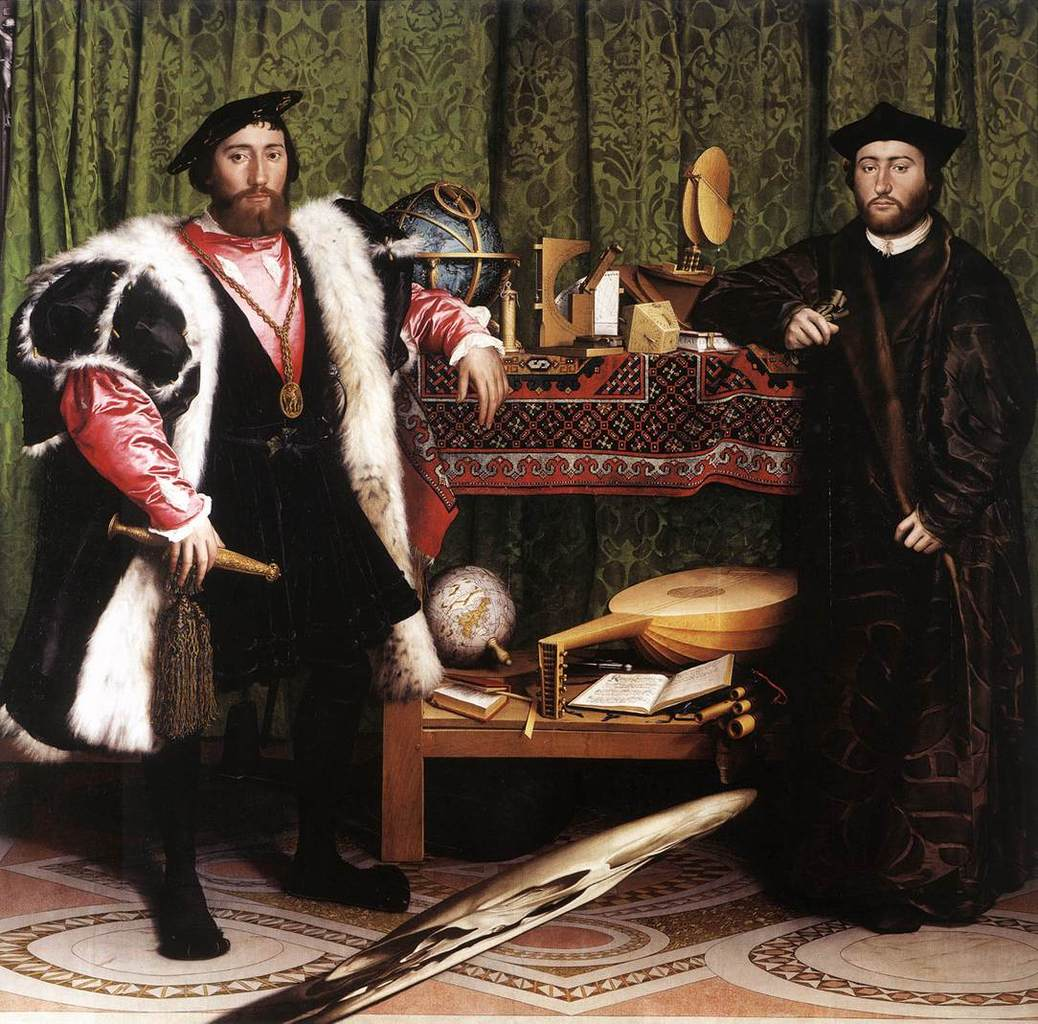
\includegraphics[scale=0.7]{image/ambassador.jpg}
%	\caption{Les ambassadeurs de Hans Holbein le Jeune, 1533}
%	\label{fig:ambassador}
%\end{figure}
%
%Sur cette toile, on peut voir apparaître une forme étrange sur le bas de ce tableau, il s'agit d'une anamorphose d'un crâne humain. Si on regarde le tableau depuis le côté inférieur gauche du tableau, le crane est visible correctement. L'anamorphose est présente sur plusieurs supports, comme par exemple dessiné par des artistes dans certaines rues \cite{pavementArt}.
%
%Dans ce projet nous allons étudier l’anamorphose dite dynamique qui fut introduite par Solina et al. \cite{solina2007dynamic}. L’aspect dynamique de l’anamorphose consiste à ne pas appliquer une déformation statique de l’image, pour laquelle il faut se placer à un point de vue particulier pour obtenir visuellement l'image non déformée, mais déformer l’image en temps réel en tenant compte de paramètres, tels que la position de l’utilisateur face a l’image, pour que celle-ci soit déformée mais parfaitement visible pour l'utilisateur. 
%
%L'anamorphose dynamique introduite par Solina et al. est de la distorsion d'image pour afficher des visages tout en ayant l'impression que le regard des portraits est dirigé vers l'utilisateur. Nous reprendrons donc l'idée de la déformation dynamique sans conserver l'objectif de Solina et al. qui était de garder la direction du regard du portrait vers l'utilisateur.
%
%La correction de perspective a également été mise en place pour le prototype Screenfinity \cite{Schmidt:2013:SEP:2470654.2466227} réalisé par Schmidt et al. . L'objectif de Screenfinity est d'afficher du texte déformé sur un écran géant pour que les passants puissent lire le texte tout en marchant et sans l'effet de perspective. Screenfinity utilise donc la déformation dynamique d'image en tenant compte de la position des passants et de leurs orientation de tête. Pour calculer la déformation à appliquer en fonction de la position et l'orientation des passant, il faut tenir compte de l'acuité visuelle.
%
%\section{Acuité visuelle et modèle de perception}
%
%L'acuité visuelle est la mesure de la résolution spatiale du processus visuel, autrement dit de l'oeil humain. La vision binoculaire est un mode de vision dans lequel les deux yeux sont utilisés simultanément \ref{fig:acuite}. 
%
%\begin{figure}[!ht]
%	\center	
%	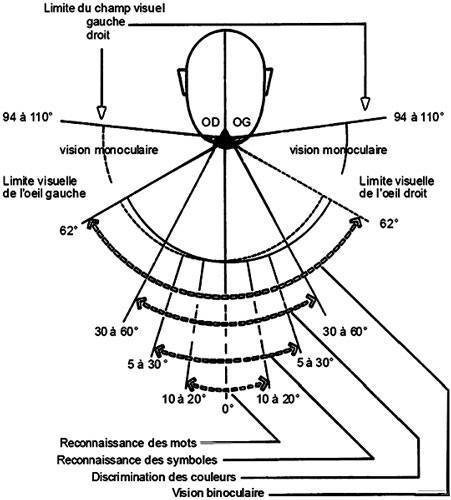
\includegraphics[scale=0.4]{image/acuite.jpg}
%	\caption{Représentation des différents champs de vision de l'être humain.}
%	\label{fig:acuite}
%\end{figure}
%
%Les humains ont un maximum de champ de vision horizontal de $\simeq$180\degres  environ avec les deux yeux, chaque oeil ayant un champ d'environ 150\degres  (90\degres  du côté temporal et 60\degres  du côté nasal) de ce qui permet d'avoir un champ de vision binoculaire de 120\degres  flanqué de deux champs monoculaires d'environ 40\degres. Il donne une sommation binoculaire augmentant la capacité de détecter des objets faiblement lumineux. Il permet une vision stéréoscopique permettant une appréciation précise des distances. En effet, la vision binoculaire est normalement accompagnée de la fusion par le cerveau des deux images perçues par les yeux en une seule mais qui permet d'avoir conscience des distances. 
%
%La vision binoculaire est donc la vue globale qu'un être humain peut avoir. Ce champs de vision sera utilisé pour calculer comment effectuer la déformation de l'image.  
%
%L'acuité visuelle ainsi est également importante dans le cas ou la densité d'affichage est élevé et que l'on souhaite lire à distance des informations. L'une des idées mise en avant est une loupe, ce qui permettra à l'utilisateur de lire à distance l'information voulue sans avoir à utiliser l'outil de déformation d'image qu'il utilisera lorsque celui s'approche de l'écran.
%
%\section{Confort visuel à distance, magnifying glass}
%
%Comme dit précédemment les écrans sont de plus en plus grands et leurs résolutions sont également de plus en plus élevées. Trois problèmes liés à l'augmentation du nombre de pixel présent par unité d'espace, autrement appelé pixel per inch (ppi) sont présentés selon Agarwal et al. \cite{Agarwal:2013:WSA:2578048.2578052}. Sur les trois problèmes identifiés deux nous concernent directement pour l'utilisation distante des grands écrans.
%
%Le premier problème étant que la plupart des applications, les systèmes d'exploitation et plus généralement les interfaces graphiques ne sont pas adaptés pour des résolutions élevées. Ce fut le cas des écrans "Retina" (220 ppi) d'Apple qui ont dû forcer certaines applications à se mettre à jour car inadapté pour une telle résolution, habituellement comprise entre 72 et 110 dpi. Ensuite vient le problème lié à la vision des utilisateurs. En effet les utilisateurs ayant des troubles de la vision, tels que les daltoniens ou encore les personnes âgées, souffrent des mêmes problèmes face à des écrans avec de grandes résolutions d'affichages. Ces problèmes sont des incapacités à lire correctement du texte ou encore à voir avec précision l'ensemble des images affichées à l'écran.
%
%Pour palier à ces problèmes d'affichage trop petit une solution fut d'utiliser les loupes \cite{Kline:1995:IGA:223904.223919}, autrement appelées magnifying glass.
%
%\begin{figure}
%    \centering
%    \subfigure[]{\label{sub1} 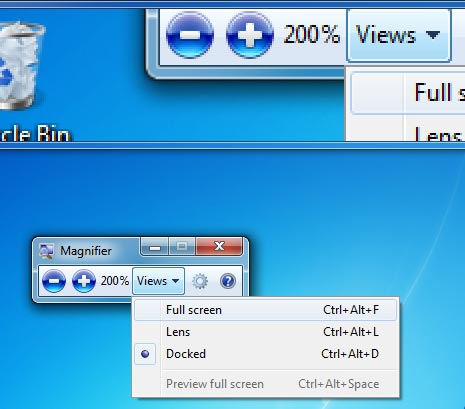
\includegraphics[scale=0.4]{image/loupeWindows.jpg}}
%    \subfigure[]{\label{sub2} 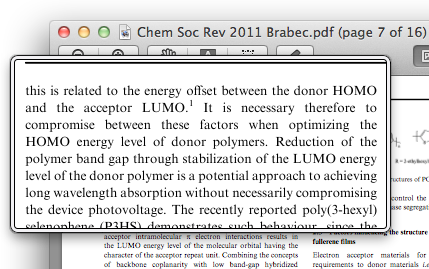
\includegraphics[scale=0.4]{image/loupeMac.png}}
%    \caption{Aperçu des loupes implémentés dans \subref{sub1}Windows et \subref{sub2}Mac OS X.}
%	\label{fig:loupeDemo}
%\end{figure}
%
%Parmi les loupes existantes et implémentées dans les systèmes d'exploitation modernes, la plupart occupent l'ensemble de l'écran ou cachent certaines parties autour de la loupe, voir figure \ref{fig:loupeDemo}. Cela à pour effet de perdre une partie des informations se trouvant sous les bords de la loupe. Pour les loupes qui occupent une plus grande partie de l'écran, cela a pour effet de perdre encore plus d'informations car si l'utilisateur n'a pas connaissance de son environnement graphique, il doit parcourir l'ensemble de l'écran pour pouvoir s'y repérer et interagir. 
%
%Pour garder une vue globale de l'environnement graphique de nombreuses loupes ont étés expérimentés \cite{Carpendale:2004:AHM:1029632.1029645}. L'une des loupes qui ré-apparaît souvent dans la littérature est la loupe fisheye
%
%Dans le domaine de l'interaction homme machine la question du zoom fisheye a souvent été étudié \cite{Shneiderman:1986:DUI:6682, Ware:1995:DIM:223355.223749, Cockburn:2009:ROZ:1456650.1456652} et mis en avant pour montrer l'avantage de cette technique en ce qui concerne la mise en focus de certains éléments. L'une de ses utilisations la plus connue est sur le dock de max OS X. L'effet fisheye est une distorsion de l'image qui apporte un gain de performance \cite{Bederson:2000:FM:354401.354782, Furnas:1999:FVN:300679.300769, Gutwin:2002:IFT:503376.503424, Gutwin:2003:FGL:642611.642648} lorsque l'utilisateur souhaite parcourir des données et se concentrer sur une de ces données. Cependant lors d'une sélection, l'effet de distorsion affecte positivement le nombre d'erreurs \cite{Gutwin:2002:IFT:503376.503424}. L'effet fisheye apporte donc une loupe dite contextuelle.
%
%Un des autres types de loupes souvent mis en avant est la loupe dite de lecture. Cette loupe comme visible dans la figure \ref{fig:loupeDemo}, est souvent bornée et cache une partie des informations comme expliqué ci-dessus. XXXXXXXXXX \cite{} qui a expérimenté un ensemble de loupe montre qu'une loupe de lecture avec une distorsion d'image sur les bords de la loupe et un ratio fixe de déformation appliqué autour du centre de la loupe peut correspondre à ce qui est actuellement fait pour les loupes de lecture.
